\documentclass[main.tex]{subfiles}
% \nomenclature[A]{GPR}{Ground Penetrating Radar}%

\begin{document}
\chapter{Project Management}
\chaplabel{projectManagement}
%\textcolor{red}{This chapter provides a high level overview of various management aspects of the project with an overview of the project goal and  any changes that occurred since the Preliminary Report. The main stakeholders involved with the project are then identified, and their roles are explained. The division of the project workload amongst the team members is shown in the work breakdown structure, and a final Gantt chart is presented to demonstrate the workload and organisation over the time-line of the project. A risk assessment is also presented and any unforeseen shortfalls discussed. Finally, the budget for the project is presented and analysed showing the funding breakdown for the project.}

Project management provides a high level overview of the management aspects of the project including the project goal and any changes that have have been made since the Preliminary Report. Division of the project workload amongst the team members was critical for project completion and is determined through a work breakdown structure. A final Gantt chart was drafted to demonstrate the workload and organisation over the time-line of the project. A risk assessment was also conducted and any unforeseen shortfalls discussed as well as an analysis of the budget and expenditure for the project.

\section{Path to project completion}
% Talk about deliverables and milestones as well, taking some details from below:
%%%%%%%%%%%%%%%%%%%%%%%%%%%%%%%%%%%%%%%%
% The deliverables for the project in semester 1, 2016 are the project charter and preliminary report. These deliverables were due on 24th March and 3rd June, 2016, respectively. 
% Deliverables for semester 2, 2016 include, and is not limited to, seminar presentation, final report and  Ingenuity expo. The tentative dates for these deliverables are 20th to 22nd September, 21st October and 27th to 28th October, 2016, respectively. 
% In addition, a deliverable for a computer simulation of the platform automation and navigation is required by the date of the Ingenuity expo as this will be displayed in lieu of a platform demonstration. There are further deliverables and milestones listed in \Chapref{ganttChart} and will be modified accordingly should the need arise. 
%%%%%%%%%%%%%%%%%%%%%%%%%%%%%%%%%%%%%%%%

The initial concept proposed in the project charter was to utilise a hovercraft for landmine detection, however, a change of scope to involve different land based vehicles was necessary to ensure project specifications were met. The change in scope and direction of the project was a result of extensive literature reviews on landmine detection methods, automation and navigation software, and platform systems. The revised project direction was to use a wheeled platform and a multi sensor system. Project sponsorship through the DSTG was achieved whereby equipment loaning, technical assistance, and funding was given. The GPR, metal detector, and the quad bike as well as \$16,500 of project funds were received.

With the project heavily incorporating both software and hardware development, project and team management was crucial for the timely completion of the objectives. This was achieved through assigning individuals champion roles for each of the systems. The systems encountered throughout the project were software development for the automation and navigation of the quad bike, wireless communications, hardware modification, sensor analysis, and whole system testing. Champions were tasked with delegating smaller tasks and ensuring forward progress was being made on each system.

Modifications to the Gantt chart constructed from the Preliminary Report included the change in scope of the project from the hovercraft to the quad bike. Further subsystem modifications and testing was required to be added which were not present for the hovercraft. A delay in platform delivery meant that advancements in software development for the automation of the platform were able to be achieved and completed ahead of schedule. Once delivery of the platform was accepted, progress was able to be achieved swiftly due to the reduced software workload allowing for more focus on the quad bike.

Testing of the sensors in differing soil properties and depths allowed for comprehensive knowledge of the outputs over targets, allowing for the development of the algorithms necessary to determine the probability of whether an object is a landmine or not, and the classification of landmines. Modifications to the detection depths highlighted in the Preliminary Report were necessary after sensor testing and communications with the DSTG. A maximum depth of 150 mm was selected as this was the maximum testing depth used by the DSTG. 

Navigation tests were conducted with the quad bike to fine tune all electronic control systems. Errors with the wheel encoder output were experienced delaying testing to try and rectify the issue. The increasing steering angle was also found to require more throttle to maintain the speed but due to the erroneous readings from the wheel encoder, distances could not be confidently determined. This lead to inaccurate navigation and positioning as the angle turned by the quad bike did not match the angle the positioning system estimated. Further modifications to the objectives include reducing the number of test requirements for the platform as there was limited time to incorporate all the aspects initially considered.  

Primary objectives that were achieved for the project can be broken down into software, platform, hardware, and sensor systems. for the platform and hardware, the objectives achieved were the modification of a platform for automation, remote operation of a platform, and the design and build of a sensor mount to adhere to the sensor requirements. For the software objectives, achievements included; development of a virtual platform, wireless communication and information display in real time on a hand held device, and automation and navigation of a platform. For the sensors, the achieved objectives include algorithm development for landmine detection, reduction in false positives, landmine identification and classification, and clutter screening. The objectives that were unable to be completed were the implementation of a physical landmine marker and the installation of a live feed camera, however progress was made.

\section{Stakeholders}

The stakeholders of the project remain largely the same as in the project charter, except the DSTG is now listed as a project partner and sponsor. \Tabref{stakeholders} shows all contributing members, and describes the roles they fulfil in the project.  

\nohyphens{	% Stop hyphenation in table
\begin{longtable}{L{0.2\textwidth} L{0.25\textwidth} L{0.45\textwidth}}
\caption[Stakeholders]{Stakeholders of the project.}\tablabel{stakeholders}\\ \toprule
\textbf{Members} & \textbf{Roles} & \textbf{Description}\\ \midrule\endfirsthead 
\caption[]{Stakeholders of the project (continued).}\\ \toprule
\textbf{Members} & \textbf{Roles} & \textbf{Description}\\ \midrule\endhead

Peter Dawson & Project Manager, Document Manager & The project manager is responsible for the overall management of the project. Their tasks involve communicating with the supervisor, group members, project sponsor and other external parties. Additionally, they are responsible for assignment of tasks and chairing of meetings. The document manager is responsible for document collation and data backup. \\ \midrule

Jonathan Targett & Technical Manager & The technical manager’s responsibility is the overall management of the technical aspects of the project. The technical aspects may include procurement mechanical resources, electronic resources and other materials for the project.\\ \midrule

Rahul Kalampattel & Safety Manager & The safety manager is responsible for lloking after the safety aspects of the project. This includes conducting risk assessments, providing a safe operating procedure (SOP), overseeing the completion of such documents and liaising with the necessary third parties to provide relevant safety information.\\ \midrule

Racquel Punu & Secretary, Test Manager & The secretary is responsible for the administrative requirements of the project, including producing meeting minutes, and submission of documents through MyUni. The test manager is responsible for overall management of any testing conducted on systems and their components as required.\\ \midrule

Harrison Vince & Treasurer, Manufacturing Manager & The treasurer is responsible for managing finances within the project. The manufacturing manager is responsible for overseeing any manufacturing processes undertaken, and dealing with other design related issues.\\ \midrule

Dr Maziar Arjomandi & Project Supervisor & Supervises student members and guides them accordingly.\\ \midrule

DSTG & Project Partner and Sponsor & Supports the project and project members in providing expertise, loaning of equipment, and funding. A research agreement entitles the Project Partner to share in all knowledge gained over the course of the project.\\ \bottomrule

\end{longtable}}

Minor stakeholders include, but are not limited to, the mechanical and electrical engineering workshop staff, School of Mechanical Engineering administration staff, honours project coordinator and others as deemed necessary by the project members. Communication between all stakeholders includes, but is not limited to, email, mobile messages, phone calls, and social media. %Added because we missed it last time. 

\section{Work breakdown structure and Gantt chart}
The Work Breakdown Structure and Gantt chart were modified from the preliminary report as necessary due to the increase in project workload and objectives as the project advanced. The time line for the GPR data acquisition and software development had to be postponed due to a faulty electrical component that rendered the system inoperable. A replacement part took a long period of time to source, however, progress was not hindered by the set back. The final versions for the work breakdown structure and Gantt chart are attached in \Chapref{WBS,ganttChart} respectively.  


\section{Risk management}
This section deals with the management of the various risks associated with the project. In \secref{safety}, safety risks are identified through a formal risk assessment. In \secref{risk}, project difficulties are described. An extensive list of risks to project failure, as well as consequences, controls and potential recovery methods, are presented in \Chapref{riskFailureApp}. 

\subsection{Safety risks}
\seclabel{safety}
Safety risks refer to those hazards that may adversely affect a person involved in the operation of the landmine detection platform. After performing a formal risk assessment, a number of hazards were identified, as listed below with the risk level in brackets:
\begin{itemize}
\item Caught between moving machinery (Low)
\item Caught on rotating parts (Low)
\item Contact with chemicals, fumes or gas (Low)
\item Contact with electricity or potential for electric shock (Medium)
\item Contact with hot object or friction burn (Medium)
\item Entangled on moving machinery (Low)
\item Exposure to noise (Low)
\item Exposure to non-ionising radiation (Low)
\item Struck by vehicle (Medium)
\end{itemize}
These hazards, as well as control measures, are described further in \Chapref{riskAss}. In order to minimise the likelihood of risks, several SOPs were developed. The latest iteration of the SOP, covering external activities using the quad bike with the sensor suite mounted, is also presented in \Chapref{riskAss}. This document MUST be consulted before operating the quad bike. 
\nomenclature{SOP}{Safe Operating Procedure}% 

\subsection{Project difficulties}% Risks of project failure}
\seclabel{risk}
Many difficulties were experienced throughout the course of the project. These encompassed the understanding of the sensor outputs and the development required to analyse complex sensor signals as well as the automation and communications with the quad bike. Misjudging time frames to acquire equipment, process risk assessments, and assess safety requirements also contributed to project time line delays.

Developing an understanding of complex sensor systems and outputs as well as software development for the analysis and fusion of sensor signals was taxing and time consuming. Extensive tests and trials had to be conducted for each sensor system to be able to draw similarities between signal outputs to find the required metrics to base the detection algorithm on. These tests were time intensive and at times inconclusive, requiring repeat tests to be carried out. One of the ongoing difficulties with the sensory systems was the varying signal output for the GPR due to changing soil parameters. Another problem faced was the detection of composite landmines as the signals produced by them are very similar to the soils that were used for testing. 

Difficulties experienced with the quad bike were associated with the communications and control of the system as a whole. Issues with the communications between the Ardiuno and the main computer were intermittent resulting in unsafe conditions to test the quad bike until they were rectified.

Initially it had been planned to perform navigation testing at a larger ground available at the DSTG. However, a redevelopment of this site which overlapped our testing schedule meant that this site was not available to the project. As a result, testing of the quad bike was constrained to a small enclosure that limited the range of tests which could be performed on the system under autonomous navigation. Numerous safety measures and precautions that were required for use of the publicly accessible site also delayed and limited the extent to which testing could be performed. Extensive bunting, barricades and a variety of kill switches and emergency stops were implemented.

The issues that could result in project failure were predicted in \Chapref{riskFailureApp} at the onset of project. They provided an overview of the possible routes the project could fail along as well as the necessary controls and ways to recover the issue. 
During the project, all possible events that were predicted occurred to some extent but were rectified allowing for the project to continue. 
The first issue encountered was upon delivery of the platform as it was not in a functioning state. This resulted in it not being able to meet the operation requirements. The controls and recovery measures were implemented and all issues found promptly. The mechanical workshop was required to disassemble the carburettor to clear it while most electronics were replaced allowing the quad bike to meet operational requirements.
During the sensor testing stage, the GPR unit malfunctioned and was inoperable for a duration of two months. The consequences were that multi sensor testing  was unable to occur simultaneously resulting in testing delays. 
This issue was rectified by sourcing a new part from the CSIRO which allowed testing to continue on the sensor systems.

\section{Budget}
A number of resources were sourced and provided to support the progression of the project. They were identified as follows:
\begin{itemize}
\item School funding: The School of Mechanical Engineering provided Honours Project students with up to \$200 per student to cover approved expenses.
\item Workshop support: the workshop provided up to 40 hours of workshop time per student valued at \$50 per hour.
\item Supervisor time: The project supervisor contributed up to 32 hours towards the project via weekly one hour meetings.
\item Quad bike: Through liaising with the DSTG a remotely operated quad bike was made available.
\item Detection equipment: Through liaising with the DSTG, GPR and MD units were made available.
\item DSTG sponsorship: Through liaising with the DSTG, project sponsorship of \$16,500 was received. 
\end{itemize}
The final standing of the project was \$13,044.84 in credit with \$3,455.16 total expenditure. The group put 2294.5 hours towards the project totalling \$152,967 in labour costs thus far. See \secref{sponsorship}, and \secref{labourcosts} for further detail on sponsorship and labour costs, respectfully. A summary of the project expenditure can be seen in \Figref{expenditurebreakdown} with a detailed material list shown in \Chapref{budgetApp}.
\begin{figure}[ht]
\centering
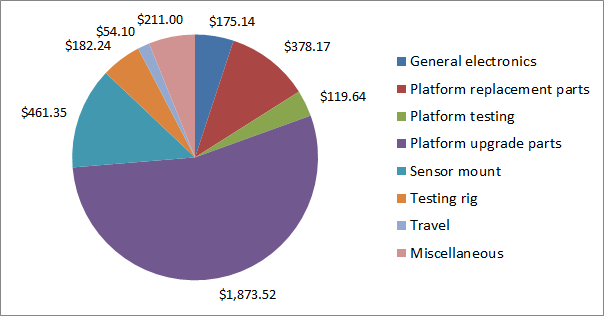
\includegraphics[]{6-ProjectManagement/expenditurebreakdown.png}
\caption[]{Expenditure breakdown}
\figlabel{expenditurebreakdown}
\end{figure}

\subsection{Sponsorship}
\seclabel{sponsorship}
It was clear from the objectives that funding would be needed to progress with the project, primarily in gaining access to expensive detection equipment and securing a mobile platform. Contact with DSTG was made and through mutual views on project outcomes, funding was granted to the value of \$16,500 as well as the supply of a remotely operated quad bike and detection equipment.

\nohyphens{	% Stop hyphenation in table
\begin{longtable}{L{0.45\textwidth} L{0.27\textwidth} L{0.18\textwidth}}
\caption{Project funding} \tablabel{funding}\\ \toprule
\textbf{Sponsor} & \textbf{Date Approved} & \textbf{Funding (\$)} \\ \midrule\endfirsthead 
\caption[]{Project Funding (continued)}\\ \toprule
\textbf{Sponsor} & \textbf{Date Approved} & \textbf{Funding (\$)} \\ \midrule\endhead
The University of Adelaide & 29/02/2016 & 1,000\\
Defence Science and Technology Group & 27/05/2016 & 16,500 \\ \midrule
\multicolumn{2}{r}{\textbf{TOTAL}} & 17,500 \\ \bottomrule 
\end{longtable}}

\subsection{Labour costs}
\seclabel{labourcosts}
To obtain a figure for the total project cost thus far, labour hours put in by each student have been tallied and included.  Each team member recorded their hourly input on a daily basis, a summarised chart is shown in \Figref{teamhours} and a detailed table can be seen in \Chapref{budgetApp}. Salaries are calculated at the rate of \$26/hr, with other direct and indirect costs included. Direct costs incur an additional 30\% on top of salary for items such as superannuation, payroll tax, workcover and long service leave. Indirect costs incur an additional 130\% on top of salary for items such as administration, technology, infrastructure, rent, phone and internet. The labour costs for the project total \$152,967.
\newpage
\begin{figure}[ht]
\centering
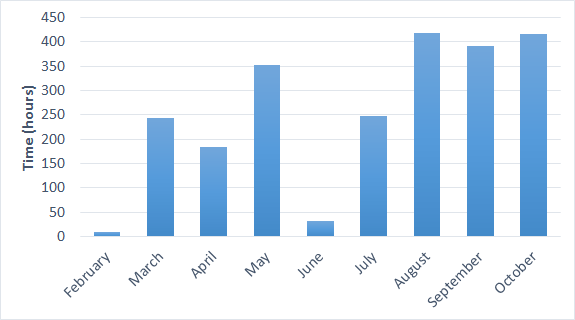
\includegraphics[]{6-ProjectManagement/teamhours.png}
\caption[]{Team hours spent on the project}
\figlabel{teamhours}
\end{figure}

\end{document}